\documentclass[a4paper, 12pt,twoside]{book}

% set the paper size and the margins
\usepackage[top = 2cm, bottom = 2cm, left = 2cm, right = 4cm ]{geometry}
\usepackage[showboxes]{textpos}
\setlength{\TPHorizModule}{10mm}
\setlength{\TPVertModule}{\TPHorizModule}
\TPMargin{2mm}
% set the header and the footnote
\usepackage{fancyhdr}
% Supress the hyphenation
\hyphenation{thatshouldnot}
% for table and equations
\usepackage{tablefootnote}
\usepackage{amsmath,amsfonts,amsthm}
\usepackage{multirow}
\usepackage{hhline}
% make a wide hat for the least-squares regression line
 \usepackage{scalerel,stackengine}
\stackMath
\newcommand\reallywidehat[1]{%
\savestack{\tmpbox}{\stretchto{%
  \scaleto{%
    \scalerel*[\widthof{\ensuremath{#1}}]{\kern-.6pt\bigwedge\kern-.6pt}%
    {\rule[-\textheight/2]{1ex}{\textheight}}%WIDTH-LIMITED BIG WEDGE
  }{\textheight}% 
}{0.5ex}}%
\stackon[1pt]{#1}{\tmpbox}%
}
\usepackage[shortlabels]{enumitem}

% knitr packages
\usepackage[]{graphicx}
\usepackage[]{color}
%% maxwidth is the original width if it is less than linewidth
%% otherwise use linewidth (to make sure the graphics do not exceed the margin)
\makeatletter
\def\maxwidth{ %
  \ifdim\Gin@nat@width>\linewidth
    \linewidth
  \else
    \Gin@nat@width
  \fi
}
\makeatother

\definecolor{fgcolor}{rgb}{0.345, 0.345, 0.345}
\newcommand{\hlnum}[1]{\textcolor[rgb]{0.686,0.059,0.569}{#1}}%
\newcommand{\hlstr}[1]{\textcolor[rgb]{0.192,0.494,0.8}{#1}}%
\newcommand{\hlcom}[1]{\textcolor[rgb]{0.678,0.584,0.686}{\textit{#1}}}%
\newcommand{\hlopt}[1]{\textcolor[rgb]{0,0,0}{#1}}%
\newcommand{\hlstd}[1]{\textcolor[rgb]{0.345,0.345,0.345}{#1}}%
\newcommand{\hlkwa}[1]{\textcolor[rgb]{0.161,0.373,0.58}{\textbf{#1}}}%
\newcommand{\hlkwb}[1]{\textcolor[rgb]{0.69,0.353,0.396}{#1}}%
\newcommand{\hlkwc}[1]{\textcolor[rgb]{0.333,0.667,0.333}{#1}}%
\newcommand{\hlkwd}[1]{\textcolor[rgb]{0.737,0.353,0.396}{\textbf{#1}}}%
\let\hlipl\hlkwb
\usepackage{framed}
\makeatletter
\newenvironment{kframe}{%
 \def\at@end@of@kframe{}%
 \ifinner\ifhmode%
  \def\at@end@of@kframe{\end{minipage}}%
  \begin{minipage}{\columnwidth}%
 \fi\fi%
 \def\FrameCommand##1{\hskip\@totalleftmargin \hskip-\fboxsep
 \colorbox{shadecolor}{##1}\hskip-\fboxsep
     % There is no \\@totalrightmargin, so:
     \hskip-\linewidth \hskip-\@totalleftmargin \hskip\columnwidth}%
 \MakeFramed {\advance\hsize-\width
   \@totalleftmargin\z@ \linewidth\hsize
   \@setminipage}}%
 {\par\unskip\endMakeFramed%
 \at@end@of@kframe}
\makeatother


\definecolor{shadecolor}{rgb}{.97, .97, .97}
\definecolor{messagecolor}{rgb}{0, 0, 0}
\definecolor{warningcolor}{rgb}{1, 0, 1}
\definecolor{errorcolor}{rgb}{1, 0, 0}
\newenvironment{knitrout}{}{} % an empty environment to be redefined in TeX

\usepackage{alltt}


% packages will be used by the 'kable' package
\usepackage{booktabs}
\usepackage{longtable}
\usepackage{array}
\usepackage{multirow}
\usepackage[table]{xcolor}
\usepackage{wrapfig}
\usepackage{float}
\usepackage{colortbl} 
\usepackage{pdflscape}
\usepackage{tabu}
\usepackage{threeparttable}
\usepackage{threeparttablex}
\usepackage[normalem]{ulem}
\usepackage{makecell}
\usepackage{xcolor}
\IfFileExists{upquote.sty}{\usepackage{upquote}}{}

% define a color for highlight
\definecolor{asparagus}{rgb}{0.53, 0.66, 0.42}
\definecolor{babypink}{rgb}{0.96, 0.76, 0.76}
\definecolor{champagne}{rgb}{0.97, 0.91, 0.81}
\definecolor{forestgreen}{rgb}{0.13, 0.55, 0.13}
\definecolor{dollarbill}{rgb}{0.52, 0.73, 0.4}

\usepackage{tcolorbox}

\tcbset{width=0.9\textwidth,boxrule=0pt,colback=champagne,arc=0pt,
auto outer arc,left=0pt,right=0p}

\setlength{\parindent}{0cm}

\begin{document}

%Deal with the headers of each chapter
\pagestyle{fancy}
\fancyhf{}
\renewcommand{\chaptermark}[1]{ \markboth{#1}{} }
\fancyhead[CE,CO]{\leftmark}
\fancyfoot[LE,RO]{\thepage}

\chapter{Two-variable data analysis}
\thispagestyle{empty}
In chapter 1, we leaned how to describe the distribution of one random variable both numerically and graphically. Most of the the real life problems are about more than one variables and their interactions. In this chapter we will learn how to model and describe the relationships between two variables.
\newpage

\section{\large{The relationship between two categorical variables}}
\vspace{0.6cm}

By reading table \ref{ExampleData}, we may suspect that the is a relation between categorical variable \textit{BASKETALL} and \textit{GENDER}. Maybe boys are more likely to play basketball than girls. How can we describe the relation between  \textit{BASKETALL} and \textit{GENDER}?\vspace{0.3cm}\\

\begin{itemize}
\item \textbf{Two-way table}\vspace{0.3cm}\\
Table \ref{Two-way table} is a two-way table describing the relationship between \textit{BASKETALL} and \textit{GENDER}.
\begin{table}[H]
\begin{center}
 \begin{tabular}{c|cccc}
\hline
\multicolumn{2}{c}{}&\multicolumn{2}{c}{BASKETBALL}&\multirow{2}{*}{Total}\\
\hhline{~~--~}
\multicolumn{2}{c}{}&\multicolumn{1}{c}{Yes}&\multicolumn{1}{c}{No}&\\
\multirow{2}{*}{GENDER}&Male&$21$&$6$&$27$\\
&Female&$5$&$20$&$25$\\
\multicolumn{2}{c}{Total}&$26$&$26$&$52$\\
\hline
 \end{tabular}
\caption{Two-way table of Gender $\times$ Basketball}
\label{Two-way table}
\end{center}
\end{table}

\item\textbf{Conditional distribution} \vspace{0.3cm}

 The \textbf{conditional distribution} of a categorical variable is defined as the distribution of this variable while the value of the other variable is fixed. \vspace{0.6cm}

 \begin{table}[H]
  
 \centering
 \rowcolors{2}{asparagus}{forestgreen}
 \begin{tabular}{ccc}
  \vspace{0.2cm}
 \textit{BASKETBALL}&Percentage of Male&Percentage of Female\\
 \hline 
% \vspace{0.2cm}
Yes&$\frac{21}{26} \approx 81\%$&$\frac{5}{26} \approx 19\%$\\
 %\vspace{0.2cm}
  No&$\frac{6}{26} \approx 23\%$&$\frac{20}{26} \approx 77\%$\\
 \hline 
 \end{tabular}
 \caption{Conditional distribution}
 \label{ConditionalDistribution}
 \end{table}
 
Table \ref{ConditionalDistribution} gives the conditional distribution of \textit{GENDER} conditioned on different different values of \textit{BASKETBALL}. For example, the conditional distribution of \textit{GENDER} among those who play basketball is that: about $81\%$ of them are boys, $19\%$ are girls.\vspace{0.3cm}\\
If a student plays basketball, this students is more likely to be a boy than a girl. Clearly, there is some association between \textit{GENDER} and \textit{BASKETBALL}.\vspace{0.6cm}

\item \textbf{Association}\vspace{0.3cm}

If the conditional distributions of a variable are different while conditioned on different values of the other variable, we say there is an \textbf{association} between those variables. Otherwise, they   are \textbf{independent(with no association)}.\vspace{0.3cm}

The conditional distributions of \textit{GENDER} are different conditioned on different values(Yes, No) of \textit{BASKETBALL}. Therefore, there is an association between \textit{GENDER} and \textit{BASKETBALL}.
\newpage

\item \textbf{Marginal distribution}\vspace{0.3cm}

If we consider the distribution of \textit{GENDER} regardless of the \textit{BASKETBALL}, we just look at the data at the right margin of tabel \ref{Two-way table}.
$$\text{Percentage of girls:}\hspace{0.3cm}\frac{25}{52} = 48\%,\hspace{0.6cm}\text{Percentage of boys:} \hspace{0.3cm} \frac{27}{52} = 52\%$$
Similarly, we can find out the distribution of \textit{BASKETBALL} regardless of the \textit{GENDER} by looking at the data at the bottom margin of tabel \ref{Two-way table}.\vspace{0.3cm}

All the distributions are \textbf{marginal distribuions}, for we only consider the data at the margin of the two-way table.

\begin{textblock}{3}(15.5, -4.5)
\textblockcolor{dollarbill}
Is it true that if two variables have no association, the marginal distributions and the conditional distributions are the same?
\end{textblock}
\vspace{0.6cm}

\item \textbf{Side-by-side bar graph} is a graph to show the relation between two categorical variables.

\begin{figure}[H]
\centering
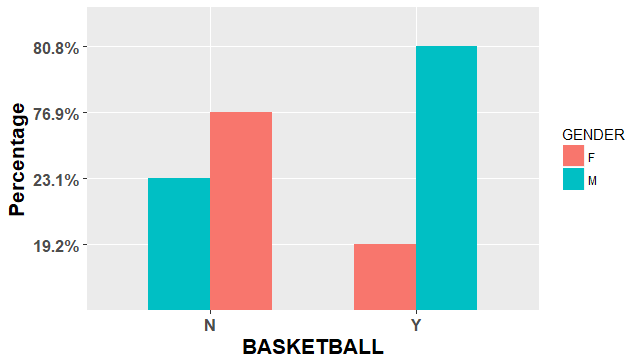
\includegraphics[scale=0.5]{Side-by-sideBarGraph.png}
\caption{Side-by-side bar graph of \textit{GENDER} and \textit{BASKETBALL}}
\label{Side-by-sideBarGraph}
\end{figure}

\item \textbf{Stacked bar graph} can play the same role as side-by-side bar graph.

\begin{figure}[H]
\centering
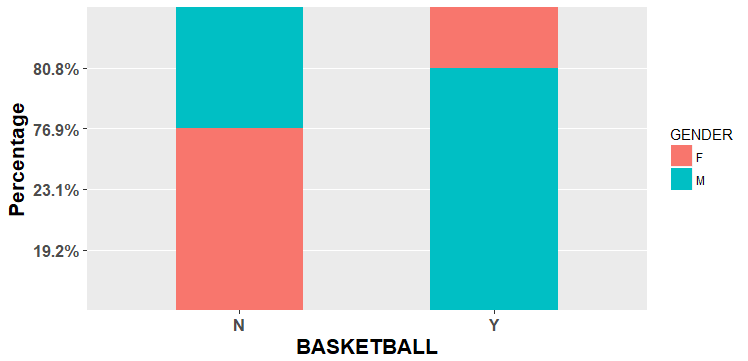
\includegraphics[scale=0.45]{StackedBarGraph.png}
\caption{Stacked bar graph}
\label{StackedBarGraph}
\end{figure}

\end{itemize}
\newpage


\colorbox{champagne}{
\begin{minipage}{\textwidth}
\large\textbf{A Titanic disaster}

In 1912 the luxury liner \textit{Titanic}, on its first voyage across the Atlantic, struck an iceberg and sank. Some passengers got off the ship in lifeboats, but many died. The two-way table below gives information about adult passengers who lived and who died, by class of travel.

\begin{table}[H]
\centering
\begin{tabular}{cccc}
\hline
&\multicolumn{3}{c}{\textbf{Class of Travel}}\\
\hhline{~---}
\textbf{Survival status}&\textbf{First class}&\textbf{Second class}&\textbf{Third class}\\
\vspace{0.3cm}
Lived&197&94&151\\
Died&122&167&476\\
\hline
\end{tabular}
\end{table}

Here's another table that displays data on survival status by gender and class of travel.
\begin{table}[H]
\centering
\begin{tabular}{ccccccc}
\hline
&\multicolumn{6}{c}{\textbf{Class of Travel}}\\
\hhline{~------}
&\multicolumn{2}{c}{\textbf{First class}}&\multicolumn{2}{c}{\textbf{Second class}}&\multicolumn{2}{c}{\textbf{Third class}}\\
\hhline{~------}
\textbf{Survival status}&\textbf{Female}&\textbf{Male}&\textbf{Female}&\textbf{Male}&\textbf{Female}&\textbf{Male}\\

\vspace{0.3cm}

Lived&140&57&80&14&76&75\\

\vspace{0.3cm}

Died&4&118&13&154&89&387\\
\hline

\end{tabular}
\end{table}

The movie \textit{Titanic}, starring Leonardo DiCaprio and Kate Winslet, suggested the following:
\begin{itemize}[\textbullet]
\item First-class passengers received special treatment in boarding the lifeboats, while some other passengers were prevented from doing so(especially third-class passengers).
\item Women and children boarded the lifeboats first, followed by the men.
\end{itemize}
\begin{enumerate}[1]
\item What do the data tell us about these two suggestions? Give appropriate graphical and numerical evidence to support your answer.
\item How does gender affect the relationship between class of travel and survival status? Explain.
\end{enumerate}
\end{minipage}
}

\newpage
\section{\large{The relationship between two quantitative variables}}

\begin{knitrout}
\definecolor{shadecolor}{rgb}{0.969, 0.969, 0.969}\color{fgcolor}\rowcolors{2}{gray!6}{white}
\begin{table}[H]
\caption{\label{SmallDataSet} Small data set}
\centering
\begin{tabular}[t]{lcc}
\hiderowcolors
\toprule
Name  & Calculus & Physics\\
\midrule
\showrowcolors
James & 75 & 74\\
Sam & 87 & 83\\
Crystal & 88 & 92\\
Evelyne & 84 & 82\\
Phoebe & 89 & 86\\
Vince & 76 & 85\\
Mike & 71 & 76\\
Lucy & 81 & 89\\
Kitty & 86 & 91\\
Owen & 88 & 82\\
Angela & 96 & 93\\
Christina & 87 & 81\\
Jamie & 84 & 80\\
Meggie & 80 & 82\\
Kevin & 97 & 99\\
Tom & 90 & 86\\
John & 81 & 88\\
Jason & 72 & 80\\
\bottomrule
\end{tabular}
\end{table}
\end{knitrout}

\begin{itemize}
 \item \textbf{Scatter plot}\vspace{0.3cm}\\
 For each student in table \ref{SmallDataSet}, there is a two dimensional coordinates (\textit{Calculus},\textit{Physics}). For example, the coordinates of 'James' is $(75, 74)$. If we draw all those coordinates out in a coordinates system, the graph is called the \textbf{scatter plot}, as shown in figure \ref{ScatterPlot}.
 
 \begin{figure}[H]
\centering
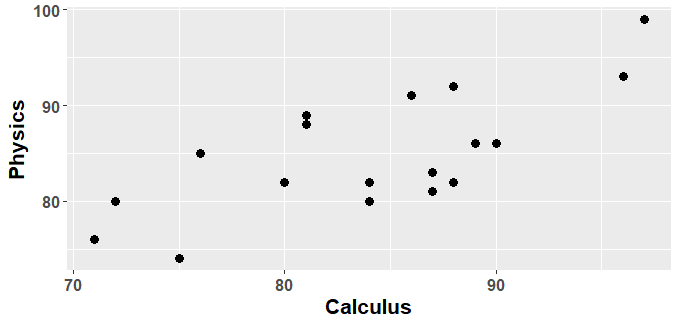
\includegraphics[scale=0.5]{ScatterPlot.png}
\caption{Scatter plot of \textit{FINAL} \textbf{vs} \textit{MID}}
\label{ScatterPlot}
\end{figure}

\vspace{3cm}

\begin{itemize}[leftmargin = 0.5cm]
 \item \textbf{Explanatory variable, Response variable}
 \vspace{0.6cm}
 
 If we want to use \textit{MID} to explain \textit{FINAL}, then \textit{MID} is called \textbf{explanatory variable} and \textit{FINAL} is called \textbf{response variable}. The explanatory variable goes to the x-axis and the response variable goes to the y-axis in the scatter plot.
 \vspace{0.6cm}
 
 \item \textbf{Direction}
 \vspace{0.6cm}
 
 The direction of a scatter plot gives a general trend, and can be described by terms \textbf{positive association} or \textbf{negative association}. If one variable increases while the other increases, those two variables have a positive association. If one variable increases while the other decreases, they have a negative association. \textit{FINAL} and \textit{MID} have a positive association according to figure \ref{ScatterPlot}.
 
  \vspace{0.6cm}
 
 \item \textbf{Form}
 \vspace{0.6cm}
 
We describe the form of a scatter plot by terms \textbf{linear} or \textbf{curved}. If the points in the scatter plot forms a linear pattern, the scatter plot has a linear form, otherwise a curved form. The scatter plot in figure \ref{ScatterPlot} has a  linear form.
\vspace{0.6cm}

\item \textbf{Strength}
\vspace{0.6cm}

Strength describes how strong is the form. Terms used to describe the strength are: \textbf{strong, moderate, weak}.
The scatter plot in figure \ref{ScatterPlot} has a strong linear relation.
\vspace{0.6cm}

\item \textbf{Outliers}
\vspace{0.6cm}

Outliers are points don't follow the pattern of the majority either in the $\textbf{x}$ direction or in the $\textbf{y}$ direction. We modify figure \ref{ScatterPlot} a little bit as shown by figure \ref{ScatterPlotOutliers}. Point \textbf{A} and \textbf{B} are outliers in the $\textbf{x}$ direction and the $\textbf{y}$ direction  respectively.

\begin{textblock}{4}(-3, 1)
Describe the scatter plot in figure \ref{ScatterPlot}.
\end{textblock}

\begin{figure}[H]
\centering
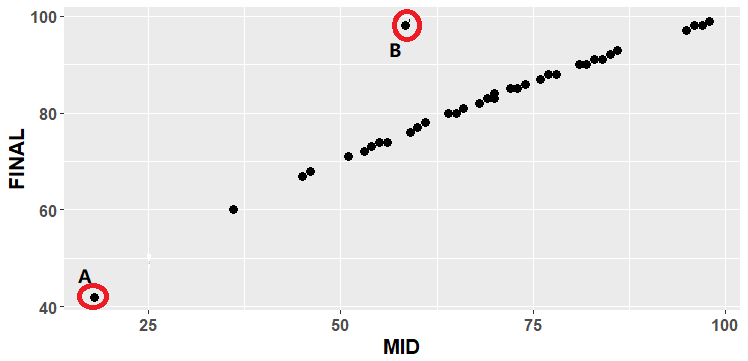
\includegraphics[scale=0.5]{ScatterPlotOutliers.png}
\caption{Outliers of a scatter plot}
\label{ScatterPlotOutliers}
\end{figure}
\end{itemize}


\vspace{1cm}

 \item \textbf{Correlation} $\mathbf{r}$
 \vspace{0.6cm}
 
 Correlation r measures the strength and the direction of the linear relationship. Suppose $\{(x_1, y_1), (x_2, y_2), \cdots, (x_n, y_n\}$ are the data points, then
 \begin{equation*}
 \begin{split}
 r&=\frac{1}{n-1}[(\frac{x_1-\bar{x}}{s_x}\frac{y_1-\bar{y}}{s_y}) + (\frac{x_2-\bar{x}}{s_x}\frac{y_2-\bar{y}}{s_y})+\cdots + (\frac{x_n-\bar{x}}{s_x}\frac{y_n-\bar{y}}{s_y})]\\
 &= \frac{1}{n-1}\sum_{i=1}^n(\frac{x_i-\bar{x}}{s_x})(\frac{y_i-\bar{y}}{s_y})\\
 &= \frac{1}{n-1}\sum_{i=1}^n z_{x_i}z_{y_i}
 \end{split} 
 \end{equation*}
 
 \begin{itemize}
  \item $\mathbf{r\in [-1, 1]}$
  $\mathbf{r>0}$ \textbf{means there is a positive association. $r<0$ means there is a negative association.}
  \vspace{0.6cm}
  
  \item \textbf{Correlation r is the measurement of the strength of the linear relationship.}
  \vspace{0.6cm}
  
  If there is a linear relationship, $|r|$ is close to 1, means the linear relationship is strong. " $|r|$ is close to 1" itself can not guarantee there is a linear relation. There may be a curved relation with $|r|$ close to 1.
  \vspace{0.6cm}
  
  $r = 0$ means there is no linear relation, but there may be a curved relationship. If  $r = \pm 1$, the scatter plot is strictly linear.
  \vspace{0.6cm}
  
  Correlation r only works on condition that there is a linear relationship. How can we tell there is a linear relationship? We will learn latter.
   \vspace{0.6cm}
   
 \item \textbf{Correlation r doesn't imply causation}
 \vspace{0.6cm}
 
 \item \textbf{Correlation r only describes the relationship between two quantitative variables and has no unit.}   
 \end{itemize} 
\end{itemize}
\vspace{0.6cm}
\colorbox{champagne}{
\begin{minipage}{\textwidth}
\textbf{Which of the following statements about correlation $r$ is true?}
\begin{enumerate}[(1)]
\item Perfect correlation, that is, when the points lie exactly on a straight line, results in $r = 0$.
\item If x increase, y increases, $r < 0$.
\item Correlation is not affected by which variable is called $x$ and which is called $y$.
\item Correlation $r$ is not affected by extreme values.
\item If the unit of the explanatory variable changes,  $r$ changes.
\item $r$ has the same unit as the response variable.

\end{enumerate}
\end{minipage}
}
\section{Least-squares regression}

Least-squares regression is a simple model of the relationship between two quantitative variables. It is simple, but it embodies the basic idea of modelling, which plays an important role in machine learning as well.

\begin{itemize}
\item \textbf{Regression lines}
\begin{figure}[H]
\centering
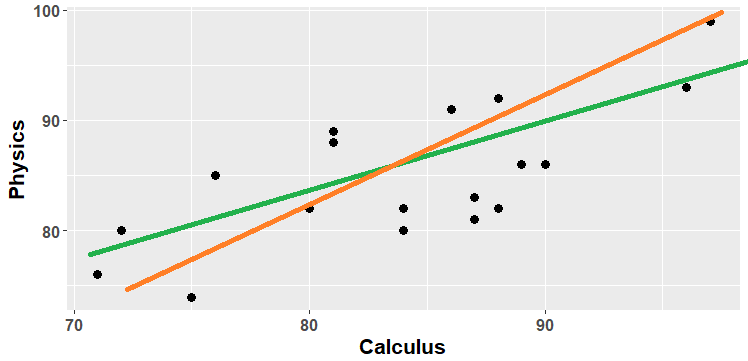
\includegraphics[scale=0.5]{LinearRegressionLines.png}
\caption{Linear regression lines}
\label{LinearRegressionLines}
\end{figure}
A regression line is a line drawn to model the scatter plot. There may be more than one regression lines as shown in figure \ref{LinearRegressionLines}. We need to set up a criteria and find the best one according to this criteria.\vspace{0.3cm}

\item \textbf{Criteria}
        
  \begin{itemize}
   \item \textbf{Residuals}
       \vspace{0.6cm}
   
   Suppose the equation for a regression line is  
   $$\mathbf{\hat{y} = a + bx}.$$ 
   $\mathbf{\hat{y}}$ is the predicted value of \textit{Physics} and $\mathbf{x}$ is the value of \textit{Calculus}. For each  value of \textit{Calculus}, we can find out a predicted value of \textit{Physics} by the equation of the regression line. Our prediction $\mathbf{\hat{y}}$ may be different from the observation $\mathbf{y}$. The difference is called \textbf{residual}.
   $$\textbf{residual} = \mathbf{y - \hat{y}}$$
  \begin{figure}[H]
\hspace{3.5cm}
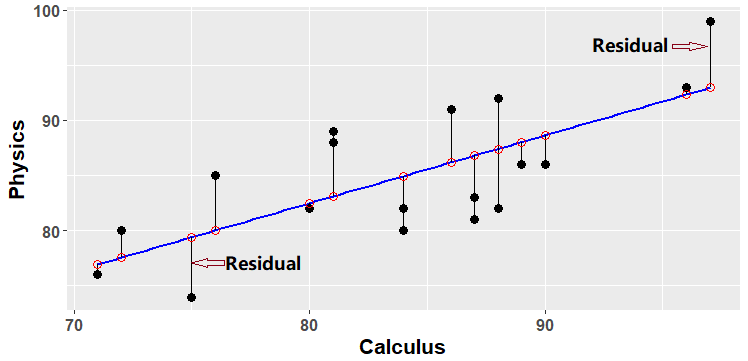
\includegraphics[scale=0.8]{VisualizingResiduals.png}
\caption{Visualizing residuals}
\label{VisualizingResiduals}
\end{figure}
A visualization of the residuals is shown in figure \ref{VisualizingResiduals}, with black dots observations and red circles predicted value, and the vertical lines connecting the red circles and the black dots represents residuals.
\vspace{0.6cm}

\item \textbf{The criteria}
\vspace{0.6cm}

We want to find a line which minimizes the sum of the squares of the residuals: $$\Sigma (\mathbf{y - \hat{y}}^2).$$
The line minimizes $\Sigma (\mathbf{y - \hat{y}}^2)$ is called \textbf{the least-squares regression line}
\vspace{0.6cm}
  \end{itemize}
 \item \textbf{Least-squares regression line}
 \begin{figure}[H]
 \begin{center}
 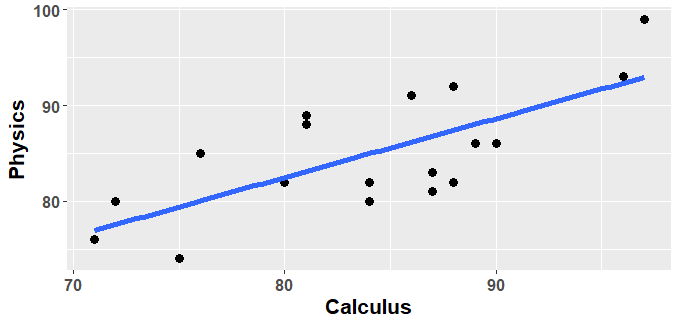
\includegraphics[scale=0.45]{LeastSquaresRegressionLine.png}
 \vspace{0.3cm}
 
 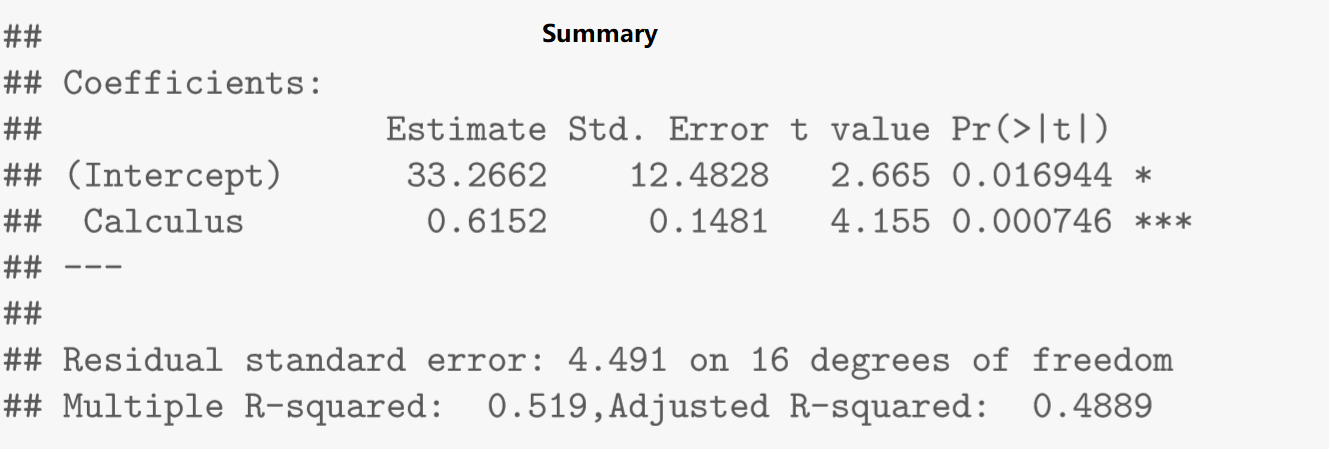
\includegraphics[scale=0.45]{SummaryLeastSquareRL.png}
 \end{center}
 \caption{Least-squares regression line}
 \label{LeastSquaresRegressionLine}
 \end{figure}
Figure \ref{LeastSquaresRegressionLine} gives a graph and a summary of the least-squares regression line. Lets read the summary.\vspace{0.3cm}

\begin{itemize}[leftmargin = 0cm]
 \item \textbf{The equation $\mathbf{\hat{y} = a + bx}$} \vspace{0.3cm}

 In the summary, $\mathbf{a}$ is the estimated coefficient of the \texttt{Intercept}: \texttt{33.2622}, and $\mathbf{b}$ is the estimated coefficient of the \texttt{Calculus}: \texttt{0.6152}. Thus the equation of the least squares regression line is $$\reallywidehat{\textbf{Physics}} = 33.262 + 0.6152 \times \textbf{Calculus}$$
 
 \colorbox{babypink}{\parbox{\textwidth}{
 The \textbf{intercept} $\mathbf{a}$ is interpreted as: when the scores of \textit{Calculus} is 0, the predicted value of \textit{Physics} is $33.3$ points. The \textbf{slope} $\mathbf{b}$ is interpreted as: when the scores of the \textit{Calculus} increases by 1 point, the scores of the \textit{Physics} will increase by 0.62 points.
 }}


\begin{textblock}{3.2}(15.5, -6)
Find the predicted value of \textit{Physics} of James and its residual. Interpret the residual.
\end{textblock}

\colorbox{babypink}{\parbox{0.9\textwidth}{
Some formulas:
$$\bar{y} = a + b\bar{x}, \quad b = r\frac{s_y}{s_x}, \quad \Sigma\textbf{residuals} = \Sigma(y-\hat{y})=0.$$
}}\vspace{0.3cm}

\item \textbf{Standard deviation of the residuals: $\mathbf{S}$}
\begin{equation*}
\begin{split}
S &= \Sigma(\textbf{residuals} - \textbf{mean of residuals})^2/(n-2)\\
  &= \Sigma(y-\hat{y})^2/(n-2)
\end{split}
\end{equation*}
\colorbox{babypink}{S gives the typical error of the predictions.}\vspace{0.6cm}

\item \textbf{Coefficient of determination: $\mathbf{r^2}$}\vspace{0.3cm}

If we know nothing about the relationship between \textit{Calculus} and \textit{Physics}. For a given value of \textit{Calculus}, a reasonable prediction of the value of \textit{Physics} is its mean, since it is the center of \textit{Physics}. In this case, the variation of the predictions from the observations is given by 
$$\frac{\Sigma(y-\bar{y})^2}{n}.$$
If the relationship between \textit{Calculus} and \textit{Physics} is given by the least-squares regression line. For a given value $\mathbf{x}$ of \textit{Calculus}, the predicted value $\hat{y}$ will be given by $\hat{y} = a + bx$. In this case, the variation of the predictions from the observations is given by 
$$\frac{\Sigma(y-\hat{y})^2}{n} = \frac{\Sigma\text{residual}^2}{n} .$$
The percentage of the variation of the response variable explained by the least-squares regression line is $$1-\frac{\Sigma\text{residual}^2}{n}\Bigg/\frac{\Sigma(y-\bar{y})^2}{n}= 1- \frac{\Sigma\text{residual}^2}{\Sigma(y-\bar{y})^2}= \mathbf{r^2} $$
This value is \textbf{the coefficient of determination}\vspace{0.3cm}

\begin{textblock}{4.6}(-3.6, -3.3)
Interpret the standard deviation of the residuals \textbf{s} and the coefficient of determination $\mathbf{r^2}$ in figure \ref{LeastSquaresRegressionLine}.
\end{textblock}

\colorbox{babypink}{\parbox{13.2cm}{$\mathbf{r^2}$ is interpreted as the percentage of the the variation of the response variable explained by the least-squares regression line relating the response variable to the explanatory variable.}}
\vspace{0.6cm}
\newpage

\item \textbf{Residual plot}

\begin{figure}[H]
\centering
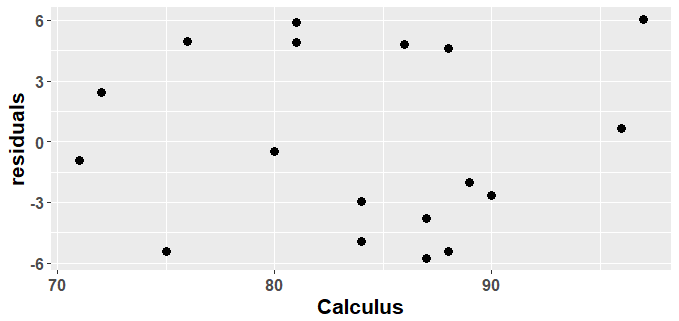
\includegraphics[scale=0.5]{ResidualPlot.png}
\caption{Residual plot}
\label{ResidualPlot}
\end{figure}
The residual plot in figure \ref{ResidualPlot} is a scatter plot of residuals against the explanatory variable \textit{Calculus}. Sometimes a residual plot may be generated by plotting the residuals against the response variable.\vspace{0.3cm}

The residual plot gives us information about whether there is any "left-over" pattern after the response variable is explained by the model. If there is no left-over pattern in the residual plot and the residuals are randomly scattered around 0, our model is appropriate. In figure \ref{ResidualPlot}, there is no left-over pattern and the residuals is randomly scattered around 0. Thus the linear model is appropriate to describe the relationship between \textit{Physics} and \textit{Calculus}.
\vspace{0.6cm}

\colorbox{babypink}{\parbox{0.9\textwidth}{Residual plot gives us information about whether a model is appropriate.}}\vspace{0.6cm}

\item \textbf{Extrapolation  and influential points}\vspace{0.3cm}

\textbf{Extrapolation} is the use of the regression line to predict the response values based on the explanatory values far out of the range from which we obtain the regression line. For the linear regression in figure \ref{LeastSquaresRegressionLine}, if a give \textit{Calculus} score is 0, the predicted value for \textit{Physics} is 33.3. \vspace{0.3cm}

\colorbox{babypink}{\parbox{0.9\textwidth}{We have to watch out for those extrapolations. Most of the time they are not accurate.}}
\vspace{0.6cm}

An \textbf{influential point} is the point that can markedly influence the result of the least-squares regression line if it is removed.\vspace{0.3cm}

\colorbox{babypink}{\parbox{12.2cm}{Outliers in the x direction are more influential.}}\vspace{0.6cm}
\end{itemize}

\newpage

\hspace{-1.5cm}
\colorbox{champagne}{
\begin{minipage}{\textwidth}
\textbf{Exercise:}

The residual plots from five different least squares regression lines are shown below. Which of the plots provides the strongest evidence that its regression line is an appropriate model for the data and is consistent with the assumptions required for inference for regression.

\begin{figure}[H]
\centering
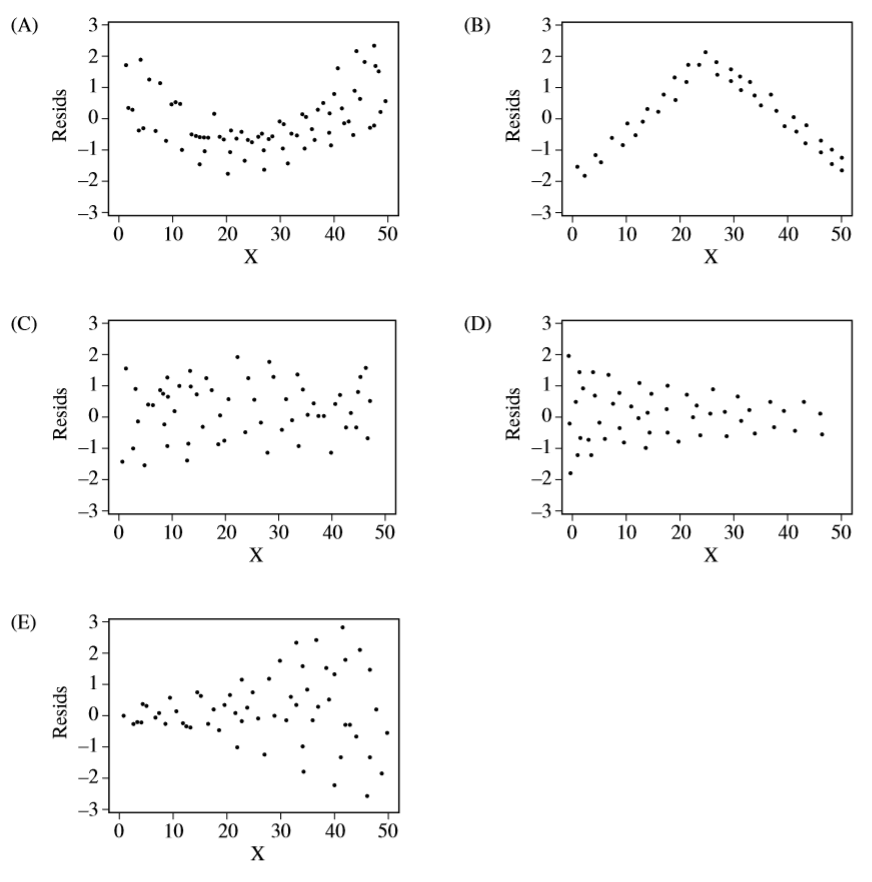
\includegraphics[scale=0.8]{Exercise2.png}
\end{figure}
\end{minipage}
}

\newpage

\item \textbf{Something more about least-squares regression}\vspace{0.3cm}

\colorbox{babypink}{
\begin{minipage}{\textwidth}
A linear model may be appropriate, but weak, with a low correlation. And, alternatively, a linear model may not be the best model(as evidenced by the residual plot), but it still might be a very good model with high $r^2$.
\end{minipage}
}

\begin{figure}[H]
\centering
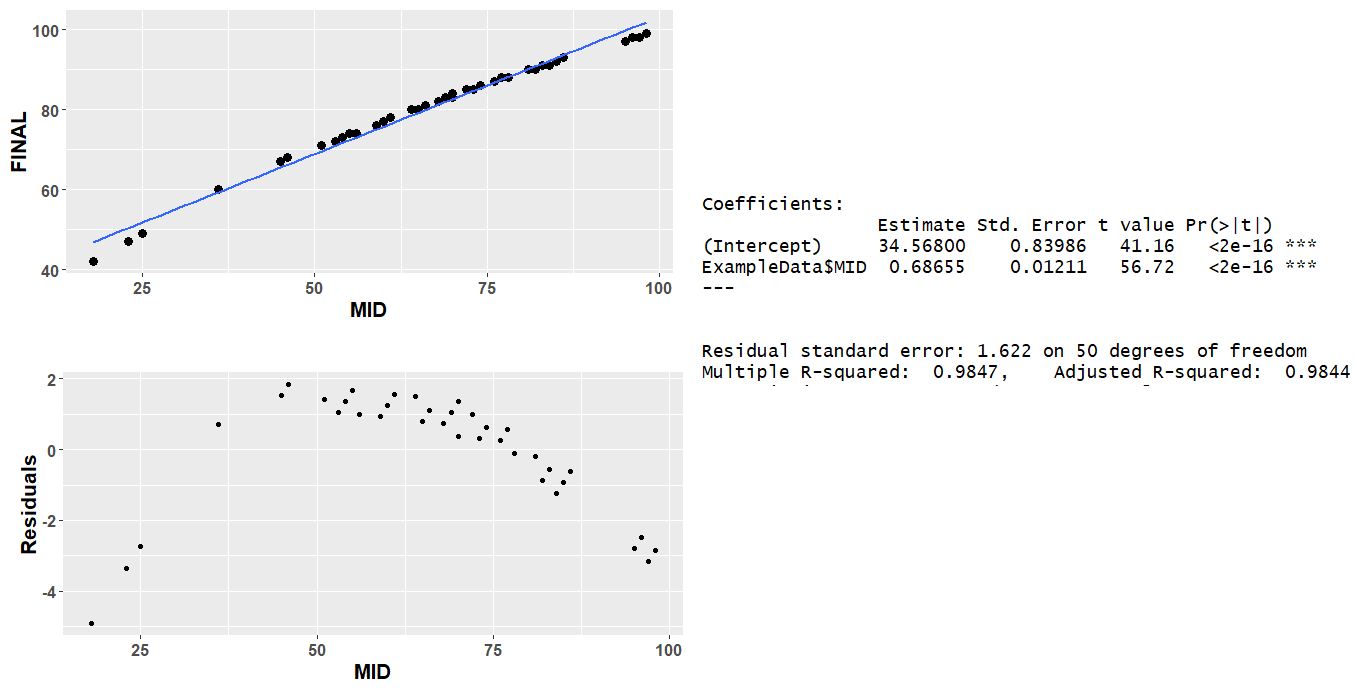
\includegraphics[scale=0.5]{Model2.png}
\caption{Linear regression of \textit{FINAL} to \textit{MID} of data in table \ref{ExampleData}.}
\label{Model2}
\end{figure}

Figure \ref{Model2} gives the output of \textbf{R packages} for the linear regression of  \textit{FINAL} to \textit{MID} of data in table \ref{ExampleData}. Clearly the residual plot is not "randomly scattered around 0" and there is a left-over pattern. Linear model is not appropriate. However, this linear model is very good with $r^2 = 0.985$, which means\textbf{ $\mathbf{98.5\%}$ of the variation of the the \textit{FINAL} is explained by our model relating \textit{FINAL} to \textit{MID}.}
\vspace{0.6cm}


In figure \ref{Model2}, \textbf{even though a lot of the variance of the response variable is explained by the least-squares regression line, there is a left-over pattern in the residual plot, and the response variable  can be further explained by some other models}. While for the model in figure \ref{LeastSquaresRegressionLine}, \textbf{there is no left-over pattern in the  residual plot, and the response variable can not be further explained.}\vspace{0.6cm}

\colorbox{babypink}{
\begin{minipage}{\textwidth}
It is important to read the output of different of different softwares in AP exam.
\end{minipage}
}

\begin{figure}[H]
\centering
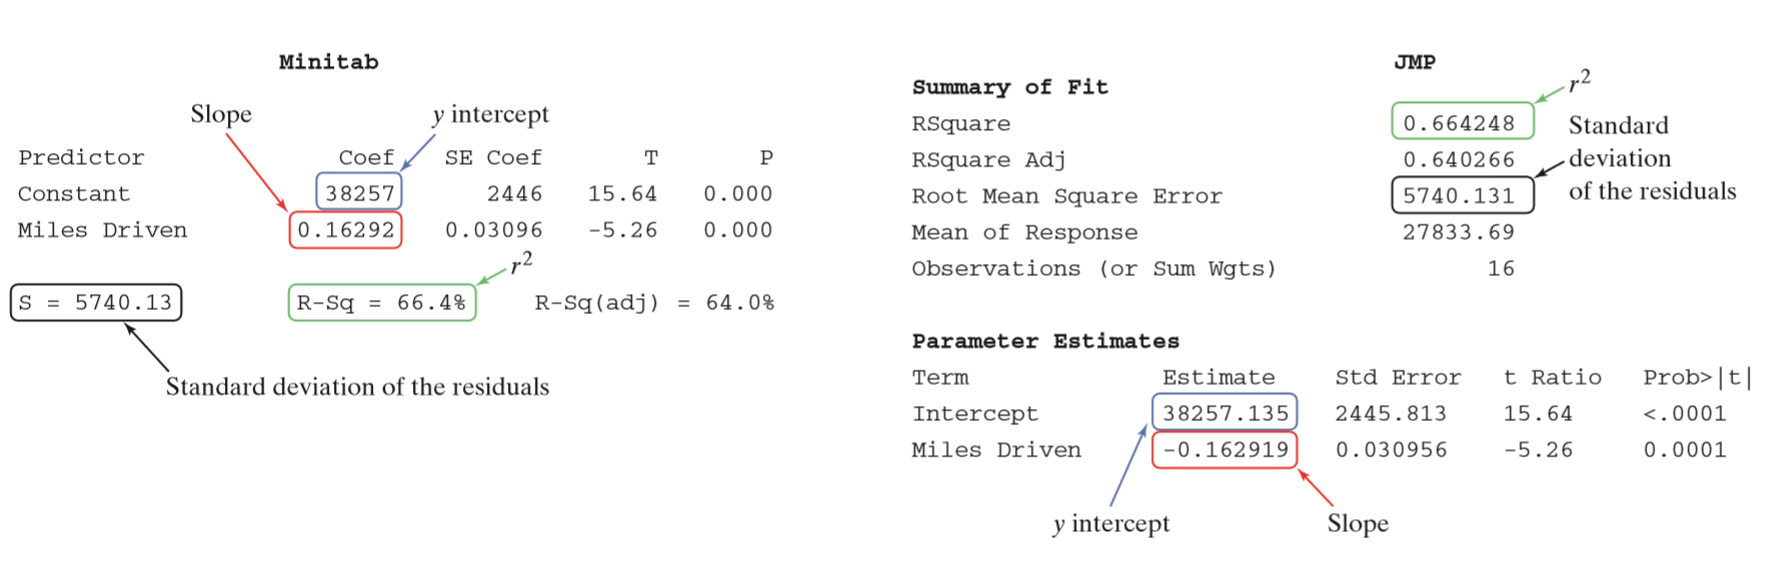
\includegraphics[scale=0.5]{OutputFormat.png}
\caption{Output formats}
\label{OutputFormat}
\end{figure}

\end{itemize}
\newpage

\colorbox{champagne}{
\begin{minipage}{\textwidth}
\textbf{Serengeti National Park}\vspace{0.3cm}

Long-term records from the Serengeti National Park in Tanzania show interesting ecological relationships. When wildebeest are more abundant, they graze the grass more heavily, so there are fewer fires and more trees grow.  Lions feed more successfully when there are more trees, so the lion population increases. Researchers collected data on one part of this cycle, wildebeest abundance (in thousands of animals) and the percent of the grass area burned in the same year. The results of a least-squares regression on the data are shown here.
        
           \begin{figure}[H]
           \centering
           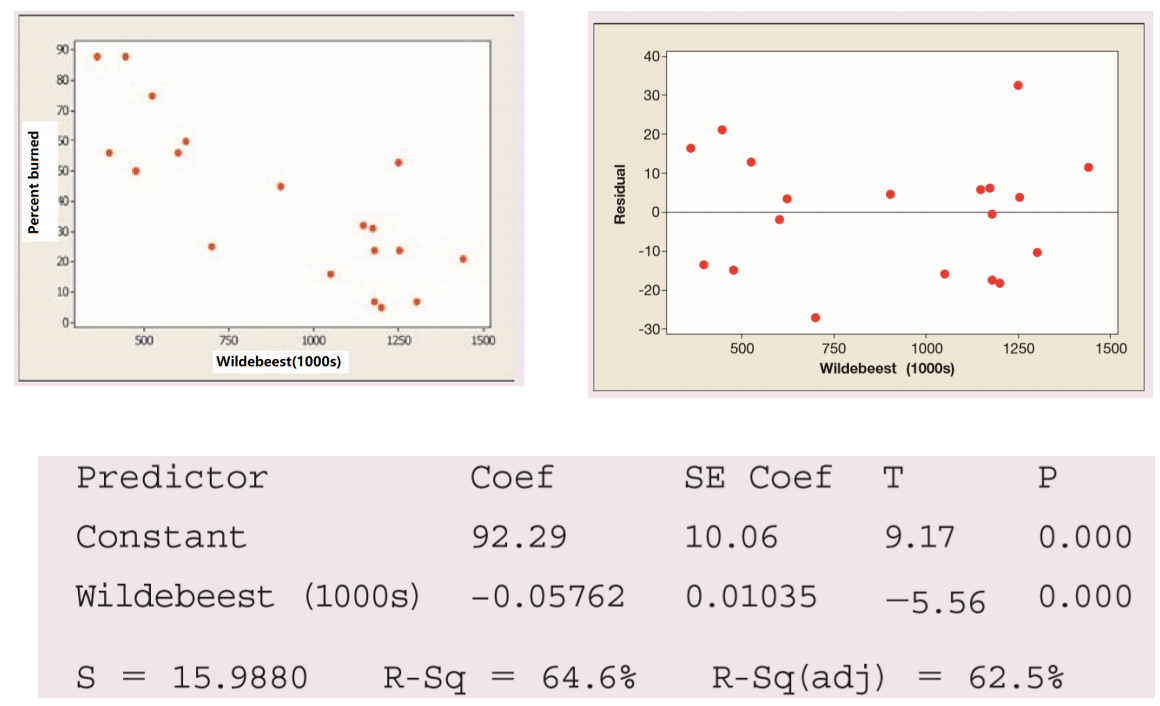
\includegraphics[scale=0.6]{LRExercise}
           \end{figure}
    
        \begin{enumerate}[(a)]
            \item Give the equation of the least-squares regression line. Be sure to define any variables you use.
            \item Explain what the slope of the regression line means in this setting.
            \item Find the correlation. Interpret this value in context.
            \item Is a linear model appropriate for describing the relationship between wildebeest abundance and percent of grass area burned? Support your answer with appropriate evidence.
        \end{enumerate}
\end{minipage}
}


\newpage






\section{Transform to achieve linearity}

In many situations, the relationship between two quantitative variables can not be described by linear models, but can be described by linear models after proper transformation. Here we will learn how to transform the \textbf{exponential models} and the \textbf{power models} into linear models.\vspace{0.3cm}

\begin{itemize}
 \item \textbf{Exponential model} \vspace{0.3cm}
 
 The exponential model is given by $$\mathbf{y=ab^x, \hspace{0.3cm} a\; \text{and}\; b \text{ are constant}.}$$ 
 \textbf{Take natural log of both sides},$$\mathbf{\ln y = \ln(ab^x) = \ln a + (\ln b)\; x}.$$
The relationship between $\ln y $ and $x$ can be described by a linear model, with intercept $\ln a$ and slope $\ln b$.
\vspace{0.6cm}

\item \textbf{Power model}\vspace{0.3cm}

The power model is given by
$$\mathbf{y=ax^b, \hspace{0.3cm} a\; \text{and}\; b \text{ are constant}.}$$ 
\textbf{Take natural log of both sides,} $$\mathbf{\ln y = \ln(ax^b) = \ln a +  b\;\ln x}.$$
The relationship between $\ln y $  and $\ln x $ can be described by a linear model, with intercept $\mathbf{\ln a}$ and slope $\mathbf{b}$.
\end{itemize}
\vspace{0.6cm}
\colorbox{babypink}{\parbox{\textwidth}{
Sometimes, we don't know whether it is a power model or an exponential model. We can draw two scatter plots to show the relationship of $\mathbf{\ln y \sim \ln x} $ and $\mathbf{\ln y \sim x}$, to see which one
 is more linear.
}} \vspace{0.6cm}

 \newpage
 
\colorbox{champagne}{
\begin{minipage}{\textwidth}
\textbf{Exercise:}

Here is the data for the nine planets in figure \ref{Planets}.

\begin{figure}[H]
\centering
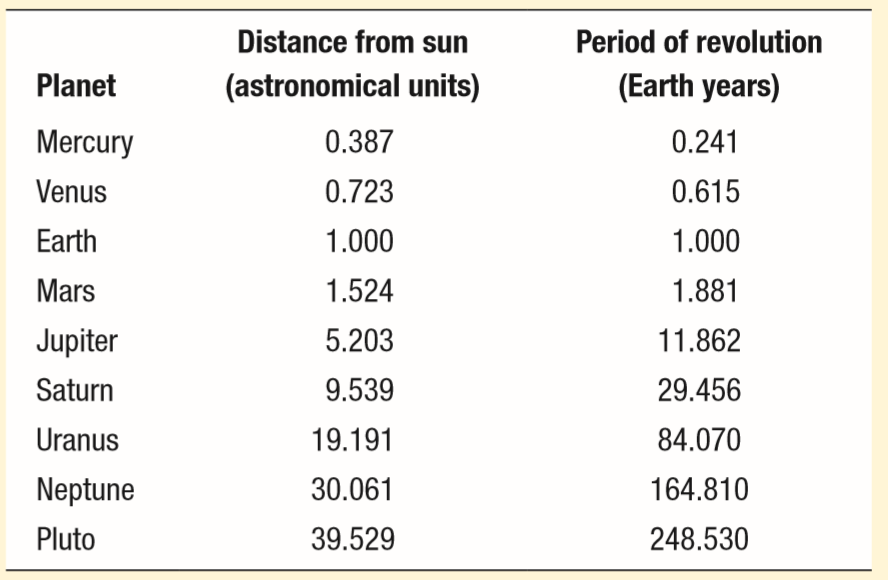
\includegraphics[scale=0.5]{Planets.png}
\caption{Data for the nine planets (\textit{Adapted from 'The practice of statistics'})}
\label{Planets}
\end{figure}
\begin{enumerate}[(1)]
\item Is power model or exponential model more appropriate to for the relationship of \textbf{Period} $\sim$ \textbf{Distance}?
\item If a new planet called Eris is discovered with distance 102.15 AU, what is the period?
\end{enumerate}
\end{minipage}
}





\end{document}